\documentclass[12pt]{amsart}
\usepackage{geometry} % see geometry.pdf on how to lay out the page. There's lots.
\usepackage{amsmath}
\usepackage{graphicx}
\usepackage{subcaption}
\usepackage{float}
\usepackage{pdfpages}


\geometry{a4paper} % or letter or a5paper or ... etc




\title{Deep Learning Homework 1}
\author{Alptekin Orbay 201700090}
\date{\today} % delete this line to display the current date


\begin{document}
\maketitle
\tableofcontents
\newpage


%%% BEGIN DOCUMENT
\section{Forward}
\subsection{Open Form}
\begin{align*}
E &= -r\log(z)-(1-r)\log(1-z) \\
z &= \sigma(\bar{z}) \\
\bar{z} &= u_1h_1  + u_2 h_2 + b_z \\
h_1 &= \sigma(\bar{h_1}) \\
h_2 &= \sigma(\bar{h_2}) \\
\bar{h_1} &= w_{11} x_1 + w_{12} x_2 + b_1 \\
\bar{h_2} &= w_{21} x_1 + w_{22} x_2 + b_2 
\end{align*}
\subsection{Compact Form}
\begin{align*}
E &= -r\log(z)-(1-r)\log(1-z) \\
z &= \sigma(\bar{z}) \\
\bar{z} &= \bold{U}\bold{h} + b_z \\
\bold{h} &= \sigma(\bar{\bold{h}}) \\
\bar{\bold{h}} &= \bold{W} \bold{x} + \bold{b_h}
\end{align*}
\section{Backward Derivation}
\subsection{Open Form}

\begin{align*}
\frac{\partial E}{\partial z} &= \frac{z-r}{z(1-z)} \quad 
\frac{\partial z}{\partial \bar{z}} = z(1-z) \quad
\frac{\partial E}{\partial \bar{z}} = z-r \\
\frac{\bar{z} }{\partial u_1} &= h_1 \quad
\frac{\bar{z} }{\partial u_2} = h_2  \quad
\frac{\bar{z} }{\partial b_z} = 1 \\
\frac{\bar{z} }{\partial h_1} &= u_1  \quad
\frac{\bar{z} }{\partial h_2} = u_2  \\
\frac{h_1 }{\partial \bar{h_1}} &= h_1(1-h_1)  \quad
\frac{h_2 }{\partial \bar{h_2}} = h_2(1-h_2)  \\
\frac{\partial \bar{h_1}}{w_{11}} &= x_1  \quad
\frac{\partial \bar{h_1}}{w_{12}} = x_2  \quad
\frac{\partial \bar{h_2}}{w_{21}} = x_1  \quad
\frac{\partial \bar{h_2}}{w_{22}} = x_2  \\
\frac{\partial \bar{h_2}}{b_1} &= 1  \quad
\frac{\partial \bar{h_2}}{b_2} = 1  \\
\frac{\partial E}{u_1} &= (z-r) h_1 \\
\frac{\partial E}{u_2} &=  (z-r) h_2 \\
\frac{\partial E}{b_z} &=  (z-r) \\
\frac{\partial E}{w_{11}} &=  (z-r) u_1 h_1(1-h_1) x_1 \\
\frac{\partial E}{w_{12}} &=  (z-r) u_1 h_1(1-h_1)x_2 \\ 
\frac{\partial E}{b_1} &=  (z-r) u_1 h_1(1-h_1) \\
\frac{\partial E}{w_{21}} &=  (z-r)  u_2 h_2(1-h_2) x_1 \\
\frac{\partial E}{w_{22}} &=  (z-r) u_2 h_2(1-h_2) x_2 \\
\frac{\partial E}{b_2} &=  (z-r) u_2 h_2(1-h_2) 
\end{align*}
\subsection{Compact Form}
\begin{align*}
\frac{\partial E}{\partial \bold{u}} &= (z-r) \bold{h^{\top}} \\
\frac{\partial E}{\partial b_z} &= (z-r)  \\
\frac{\partial E}{\partial \bold{W}} &= (z-r) ( (1-\bold{h}) \odot \bold{h} \odot \bold{u^{\top}} )  * \bold{x^{\top}}  \\
\frac{\partial E}{\partial \bold{b_h}} &= (z-r) ( (1-\bold{h}) \odot \bold{h} \odot \bold{u^{\top}} ) 
\end{align*}
\section{Experiments}

The affect of hidden unit size is indicated in figure 1. More hidden units enables fast converges as using more parameters makes the problem 
more flexible. Combining less accurate planes gives results rapidly whereas it must be too much accurate with 2 hidden units that takes more time to be learned.
\begin{figure}[H]
  \centering
  \includegraphics[width=.8\linewidth]{com.png}
  \caption{After 2000 iteration}
  \label{fig:sfig2}
\end{figure}



\begin{figure}[H]
\begin{subfigure}{.4\textwidth}
  \centering
  \includegraphics[width=.8\linewidth]{input1}
  \caption{After 1000 iteration}
  \label{fig:sfig2}
\end{subfigure}
\begin{subfigure}{.4\textwidth}
  \centering
  \includegraphics[width=.8\linewidth]{input2}
  \caption{After 2000 iteration}
  \label{fig:sfig2}
\end{subfigure}
\begin{subfigure}{.4\textwidth}
  \centering
  \includegraphics[width=.8\linewidth]{input3}
  \caption{After 3000 iteration}
  \label{fig:sfig2}
\end{subfigure}
\begin{subfigure}{.4\textwidth}
  \centering
  \includegraphics[width=.8\linewidth]{input4}
  \caption{After 4000 iteration}
  \label{fig:sfig2}
\end{subfigure}
\caption{Evolution of Planes which generates hidden units}
\label{fig:fig}
\end{figure}
\begin{figure}[H]
\begin{subfigure}{.4\textwidth}
  \centering
  \includegraphics[width=.8\linewidth]{h1}
  \caption{After 1000 iteration}
  \label{fig:sfig2}
\end{subfigure}
\begin{subfigure}{.4\textwidth}
  \centering
  \includegraphics[width=.8\linewidth]{h2}
  \caption{After 2000 iteration}
  \label{fig:sfig2}
\end{subfigure}
\begin{subfigure}{.4\textwidth}
  \centering
  \includegraphics[width=.8\linewidth]{h3}
  \caption{After 3000 iteration}
  \label{fig:sfig2}
\end{subfigure}
\begin{subfigure}{.4\textwidth}
  \centering
  \includegraphics[width=.8\linewidth]{h4}
  \caption{After 4000 iteration}
  \label{fig:sfig2}
\end{subfigure}
\caption{Evolution of Final Discrimant}
\label{fig:fig}
\end{figure}

\section{Source Code}

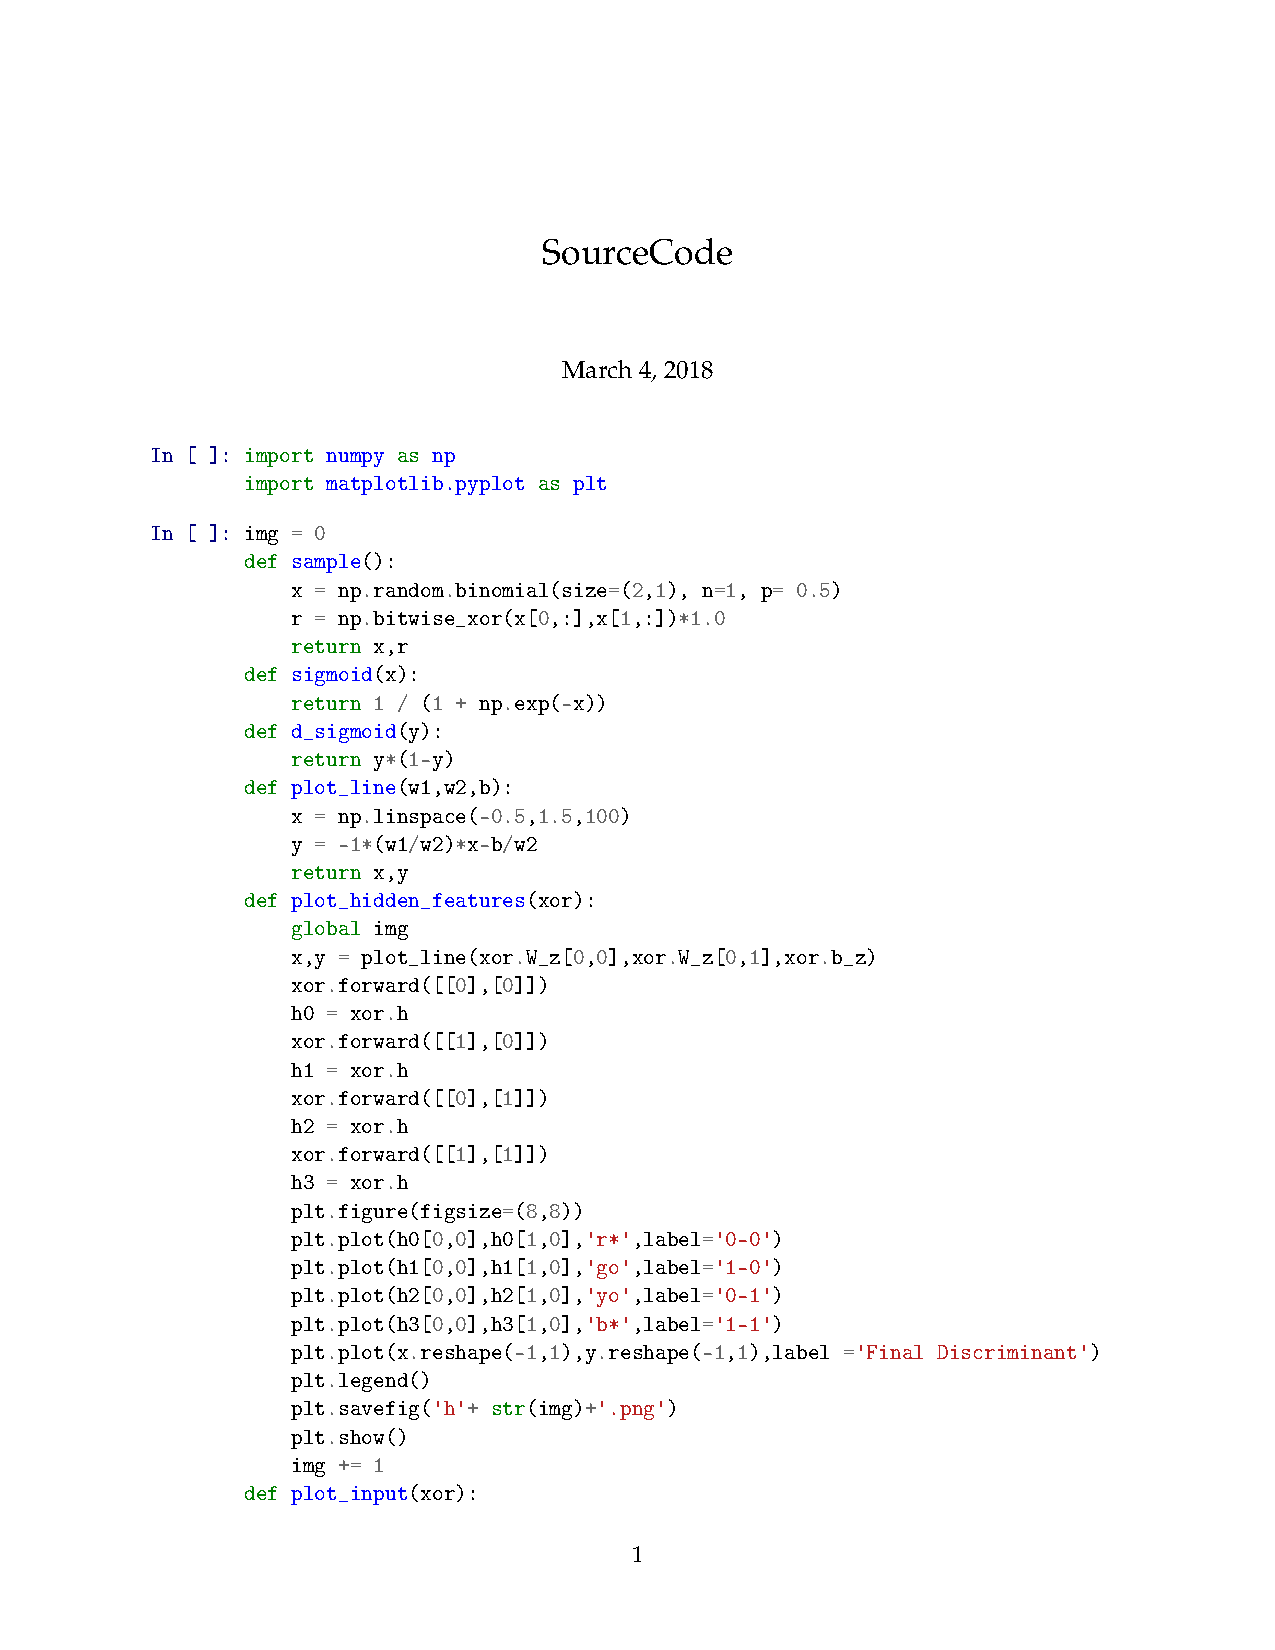
\includepdf[pages=-]{SourceCode.pdf}


\section{Additional Material}

\begin{figure}[H]
\begin{subfigure}{.5\textwidth}
  \centering
  \includegraphics[width=.8\linewidth]{h}
  \caption{Planes that generates hidden features}
  \label{fig:sfig2}
\end{subfigure}

\begin{subfigure}{.5\textwidth}
  \centering
  \includegraphics[width=.8\linewidth]{f}
  \caption{Final Plane}
  \label{fig:sfig2}
\end{subfigure}

\begin{subfigure}{.5\textwidth}
  \centering
  \includegraphics[width=.8\linewidth]{w}
  \caption{Weights}
  \label{fig:sfig2}
\end{subfigure}
\label{fig:fig}


\end{figure}

\end{document}
